% !TEX root = ../TAMU_Thesis_Main.tex

%%%%%%%%%%%%%%%%%%%%%%%%%%%%%%%%%%%%%%%%%%%%%%%%%%%%%%%%%%%%%%%%%%%%%%%
%%%                           SECTION II
%%%%%%%%%%%%%%%%%%%%%%%%%%%%%%%%%%%%%%%%%%%%%%%%%%%%%%%%%%%%%%%%%%%%%%


\chapter{PAGES WITH A FIGURE, A TABLE, AND AN EQUATION}
\section{Inserting Figures}

Figure (and table) titles should be consistent through the document. All captions should be placed either above or below the object it describes. This is done by placing the \textit{caption} in the correct place, i.e., before the {\it includegraphics} command for caption above or after for caption below).

Below is an example of a figure with the caption under the figure.
\begin{figure}[ht]
   \centering
   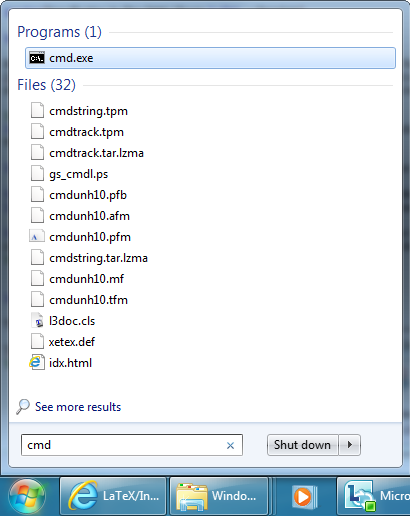
\includegraphics[width = 0.5\textwidth]{TAMUthesis_CMD_windows.png}
   \caption[The command line compiler in Windows.]{The command line compiler in Windows. It is not suggested that you compile using this method. See compilation instructions in the README.}
   \label{fig:CMD_1}
\end{figure}

\subsection{Figure placement}
When including a figure (or a table) it is important to specify where it should appear on the page. Note that when the {\it figure} environment is started of the above figure, [ht] appears after the begin statement. This tells \LaTeX\ to place the figure here in the text, or at the top of the page if it does not fit here. While \LaTeX\ will try its best to put the figure here, if the figure is too tall (i.e., it would run off the page if it were placed here), your figure will likely be pushed to the top of the next page. When using the h option, it is recommended that you specify your second preference for if the figure does not fit. If you want the figure exactly here, use the H option.

There are three other options that can be used when tell \LaTeX\ where to place figures and tables
\begin{itemize}
  \item t - top of the page
  \item b - bottom of the page
  \item p - give the figure/table its own page
\end{itemize}

It will likely take some trial and error to get your figures where you want them, but once you understand how \LaTeX\ thinks when placing figures/tables, it is very easy to get them where you want. If you are having issues with \LaTeX\ following your commands, you can try adding an exclamation mark (!) to the position (i.e., !t). I would recommend waiting until most of your text is written to start placing your figures exactly where you want them, as they will move if text is add/removed.

\subsection{Figure width/height}

If you have generate all your images to be the exact size that you want them and know they will fit within the margins of the page, then you can skip this section. If your figures are smaller/larger than you would like them to appear, continue reading see how to scale your images.

It is recommended that when specifying the width/height of images, the {\it width} or {\it height} option be used in the {\bf includegraphics} command, where {\it width} sets the width of the image and {\it height} sets the height. It is also recommend that the lengths {\it textwidth} and {\it textheight} be used when specifying the width and height of images, respectively. Factional values of these lengths can be used by simply placing a decimal number in front of the length. For example, the width of \figref{fig:CMD_1} is defined as
\begin{verbatim}width = 0.5\textwidth\end{verbatim}
which means the figure will have a width half the length of a line of text. If the figure is much taller than it is wide, you may want to specify the height.

If you would prefer to provide a scaling factor for images, you can use the {\it scale} options and specify a decimal number, e.g., scale=0.5 to make the image half its original size. Just be careful when using scaling, as images may go outside of the margins. This is why it's recommended to specify a size and allow \LaTeX\ to determine the scaling.

\subsection{Captions for figures/tables}
When adding a caption to a figure or table, the {\it caption} command is used. For \figref{fig:CMD_1}, the caption command is
\begin{verbatim}
   \caption[The command line compiler in Windows.]{The command line
   compiler in Windows.It is not suggested that you compile using
   this method. See compilation instructions in the README.}
\end{verbatim}
The text in the square brackets [] is the text that will appear in the list of figures in the table of contents, while the text in the curly brackets \{\} will appear in the caption under the figure. If the square brackets [] are not used, the text in the curly brackets \{\} will be placed in the list of figures. The same rules apply to tables using the {\it caption} command.

\subsection{Labeling figures/tables}
One of the features of \LaTeX\ is its ability to cross-reference things very easily; e.g. \figref{fig:CMD_1}. When inserting a figure, table, or even an equation, it is highly recommended that you give the object a label using the {\it label} command inside the figure, table, etc. environment. For example, \figref{fig:CMD_1} is given the label `fig:CMD\_1'\footnote{I recommend prefixing figure labels with fig:, tables with tab:, and equations with eq:. You can also label chapters, sections, etc.}. The label can be anything you want, so long as you remember what it is. Use the label whenever referencing the figure in the document and if figures are added before the figure, or the figure is moved around, the in-text reference to the figure will update to the new figure number.

To reference the figure in-text, you can use either the {\it ref} or {\it figref} command. The {\it ref} command will give you just the figure number, while the {\it figref} command will insert the figure label as well. For example, {\it ref} gives: \ref{fig:CMD_1}, while {\it figref} gives: \figref{fig:CMD_1}.

\subsection{Figure Cropping}
If you have some figures that have large margins and you do not want to remake the figures, you can crop them from the {\it includegraphics} command. Just look at \figref{fig:large_margins}. 

\begin{figure}[ht]
  \centering
  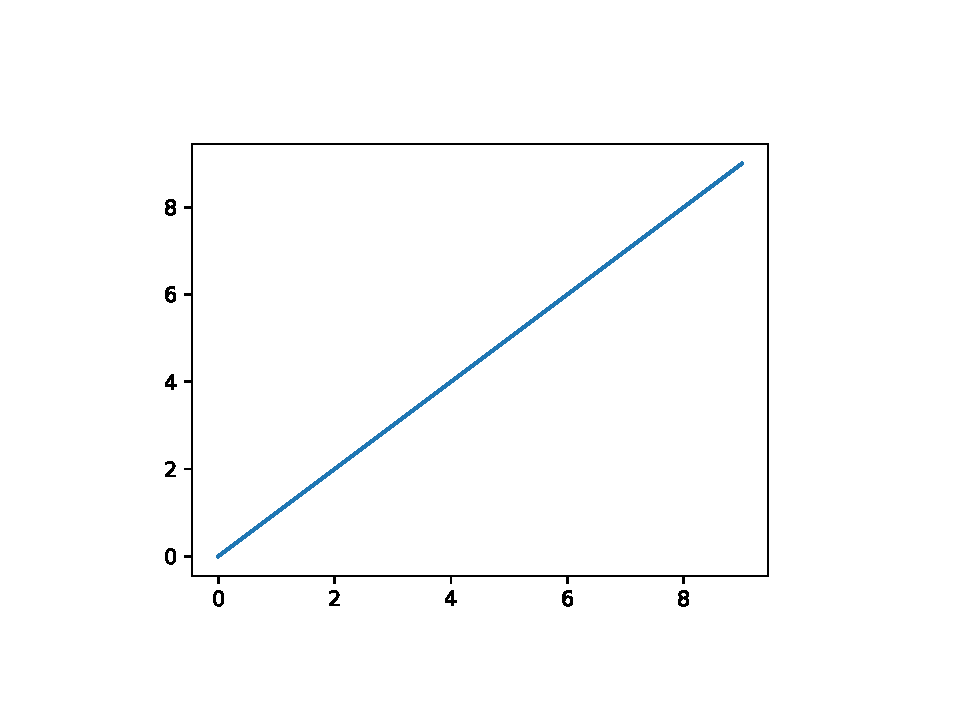
\includegraphics[width=0.6\textwidth]{figure_with_margins}
  \caption{A figure that has large margins.}
  \label{fig:large_margins}
\end{figure}

Notice that there is a good deal of white space between the bottom of the figure and the figure caption. This can be removed using the {\it trim} option in includgraphics. The option is as follows:
\begin{verbatim}
trim=0mm 0mm 0mm 0mm,clip
\end{verbatim}
where trim specifies how much of the image is to be cropped, with the four 0mm values specify how much to crop off the left, bottom, right, and top of the image (in milimeters), and clip tells includegraphics to crop the image. Figure \ref{fig:cropped_image} shows the cropped version of Figure \ref{fig:large_margins} with trim set to `0mm 15mm 0mm 15mm'; as I am only worried about the bottom (and top) margins, I did not trim the left (first value) and right (third value) sides of the image. While I used milimeters (mm) as the unit in this case, any \LaTeX\ unit of measure can be used: cm, in, pt, etc.

\begin{figure}[ht]
  \centering
  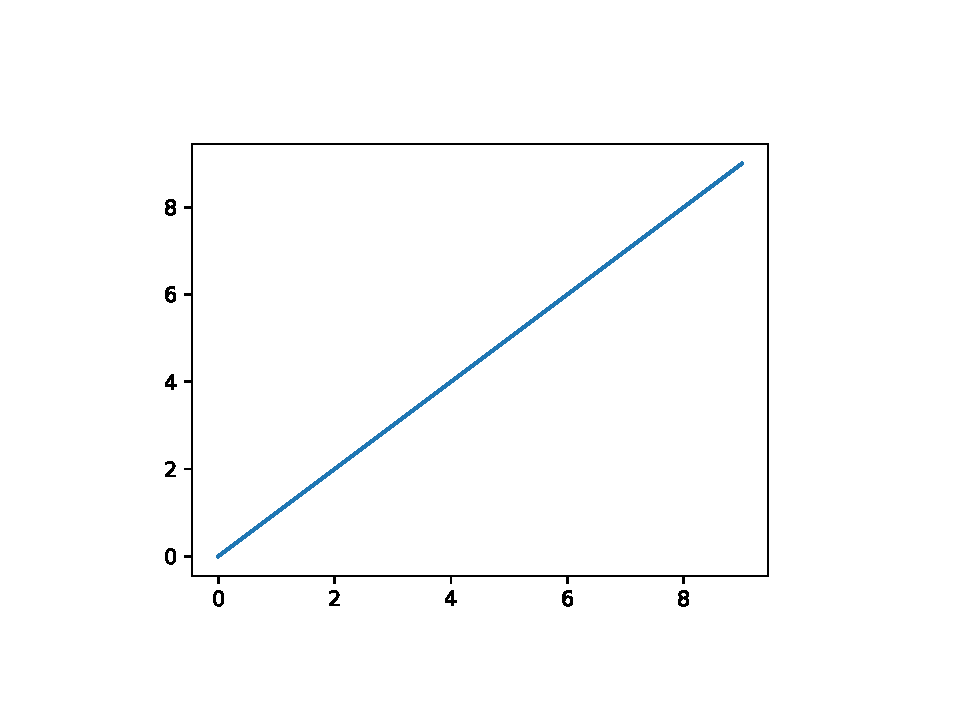
\includegraphics[trim=0mm 15mm 0mm 15mm,clip,width=0.6\textwidth]{figure_with_margins}
  \caption{As in Figure \ref{fig:large_margins}, but with the margins cropped off.}
  \label{fig:cropped_image}
\end{figure}

\figref{fig:cropped_image} is also an example of how the {\it ht} option for placement works, with the image being placed at the top of the page that it appears on.

\subsection{Continued Figures}
If you must use a continued figure, \figref{fig:continued_fig} shows and example of how to do this. All that is required is adding the {\it ContinuedFloat} command to the continued portion of the figure and ensuring that the caption command is as follows
\begin{verbatim}
\caption[]{Continued.}
\end{verbatim}


\newpage% Issued so that the next section begins on a new page
\section{Inserting Tables}

Here is a table, displaying band and auxiliary scores from the 2011 Arcadia Festival of Bands held in Arcadia, CA \cite{ARCADIA}.

\begin{table}[h!]
	\centering

	\label{Band}
	\begin{tabular}{|l|l|l|}
		\hline
		School Name & Band Score & Auxiliary Score \\ \hline
		Rancho Bernardo & 96.15 & 89.15 \\ \hline
		Mt. Carmel & 95.30 & 83.55 \\ \hline
		Riverside King & 93.85 & 91.75 \\ \hline
		Diamond Bar & 93.20 & 88.60 \\ \hline
		El Dorado & 92.80 & 95.45 \\ \hline
		Chino & 92.65 & 91.45 \\ \hline
		Henry J. Kaiser & 92.60 & 87.55 \\ \hline
		Glendora & 92.60 & 89.15 \\ \hline
		Montebello & 90.50 & 82.70 \\ \hline
		Mira Mesa & 89.65 & 91.50 \\ \hline
	\end{tabular}
	\caption{Scores from the 2011 Arcadia Festival of Bands.}
	\label{tab:band_scores}
\end{table}

The table is sorted by band score. There is more text here to demonstrate how the template handles spacing between tables and body text. When referencing tables, you can use the {\it ref} or {\it tabref} commands. {\it tabref} is similar to {\it figref} discussed above, with {\it ref} giving: \ref{tab:band_scores}, and {\it tabref} giving: \tabref{tab:band_scores}, for the above table. Also note how the table caption is in a smaller font size than the body text.

\section{Equations}\label{sec:more_equations}

The following format is recommended to be used to display equations.

%Make other examples.
\begin{equation} \label{eq:2.1}
y=c_1\cos(t)+c_2\sin(t)
\end{equation}
\begin{equation} \label{eq:2.2}
e^{it}=\cos(t)+i\sin(t)
\end{equation}

Equation \ref{eq:2.1} is the general solution to the differential equation $y''+y=0$. In the source code, the {\it ref} and {\it eqref} commands allows you to refer to an equation by a label you created. References must be made after the equation has been created; attempting to refer to an equation before it is defined results in a question mark placeholder. Some more sample equations are below. Notice the first set below is not numbered.
%%
\begin{align*}
\log (x^n) &= \log (x \cdot x \cdot \ldots \cdot x) \\
&= \log x + \log x + \ldots + \log x \\
&= n \log x
\end{align*}
\begin{equation} \label{Equ.2.3}
X^T X \mathbf{u} = X^T \mathbf{y}
\end{equation}
\begin{equation}\label{Equ.2.4}
u(x, t) = \int_{-\infty}^{\infty} G(x, \tau) \exp\left(-\frac{(t-\tau)^2}{4kt}\right) \ d\tau
\end{equation}
\begin{gather}
\mathcal{L}(f) = \int_{0}^{\infty} e^{-st} f(t) \ dt \\
\begin{split} \label{Equ.2.5}
\mathcal{F}(f) = \frac{1}{2\pi}\int_{-\infty}^{\infty} e^{i \omega x} f(x) \ dx
\end{split}
\end{gather}

You can use labels to refer to equations you create. \ref{Equ.2.5} is the \textbf{Laplace transform} used extensively in differential equations. \ref{Equ.2.3} is the matrix representation of the \textbf{normal equations} used in least-squares regression.

To have equations without labels appearing in the right margin, simply add an asterisk to the name of the environment (equation, align, etc.) when making the declaration.


\section{Theorems and Proofs: Examples}

This section will show an example usage of the theorem and proof environments, typically used for mathematics students. To use these environments, you must have the package \textbf{amsthm} declared in the preamble of your document. For this template, this is already declared in the main file. You may choose to remove this declaration if your document will not make use of theorems and proofs.

Theorems can be numbered, as the one below is, or you can force a different label to appear. For example, you can state the Bolzano-Weierstass theorem and have the names appear as the theorem label. See the examples below.

Sometimes you may have a theorem with multiple parts or multiple conditions. You can use other list environments, such as enumerate, inside the theorem environment declared to list these conditions. The final example at the end of this block shows this with the Invertible Matrix Theorem, which has several equivalent statements.

\newtheorem{thm}{Theorem}
\begin{thm}
	Suppose $f$ is of class $\mathcal{C}^1$ and $g$ is of class $\mathcal{C}^2$, and that the compact set $D$ and its boundary satisfy the hypotheses of Green's Theorem.  Then
	\[ \iint \limits_D f\nabla^2 g \ dA = \oint_{\partial D} f(\nabla g) \cdot \mathbf{n} \ ds - \iint \limits_D \nabla f \cdot \nabla g \ dA . \]
\end{thm}

\begin{proof}
	Begin with the integral of $f\nabla g \cdot n$ taken over the boundary of D.  By the second vector form of Green's Theorem,
	\begin{align*}
	\oint_{\partial D} f\nabla g \cdot n \ ds &= \iint \limits_D \nabla \cdot (f\nabla g) \ dA \\
	&= \iint \limits_D f\nabla^2 g + \nabla f \cdot \nabla g \ dA.
	\end{align*}
	
	Rearranging yields the desired.
\end{proof}

\begin{thm}[Bolzano-Weierstrass]
	Every bounded real sequence has a convergent subsequence.
\end{thm}

\begin{thm}[Invertible Matrix Theorem\footnote{This is an incomplete list.}]
	For any square matrix $A$ with $n$ rows and columns, the following are equivalent.
	\begin{enumerate}
		\item $A$ is invertible.
		\item The equation $A\mathbf{x}=\mathbf{0}$ has only the trivial solution $\mathbf{x} = \mathbf{0}.$
		\item For any nonzero $\mathbf{b}, \ A\mathbf{x} = \mathbf{b}$ has exactly one solution.
		\item The columns of $A$ form a linearly independent set.
		\item Zero is not an eigenvalue of $A$.
		\item $A$ has full rank.
		\item The determinant of $A$ is not zero.
	\end{enumerate}
\end{thm}

There is currently no set format on how propositions and theorems should be laid out in the document. The idea is to remain consistent. It is best to not customize the appearance of theorems so that they can easily be distinguished from body text - just like figures, tables, and headings.

\section{Another Table Example}
For the sake of testing the appearance of the list of tables, a second table will be displayed here. This table displays a list of some major universities and their enrollments during fall 2015. This table is sorted in descending order of enrollment.
%The savenotes environment, loaded from the footnote package
%(which in turn is loaded from mdwtools)
%allows you to use footnotes in tables, if needed.
\begin{savenotes}
\begin{table}[h!]
	\centering
	\label{my-label}
	\begin{tabular}{|l|l|l|}
		\hline
		School & City and State & Fall 2015 Enrollment  \\ \hline
		Texas A\&M University\footnote{Gig 'em!} & College Station, TX & 64,376  \\ \hline
		Ohio State University\footnote{This number describes enrollments at the Columbus campus; enrollments at regional campuses in Lima, Mansfield, Marion, Newark, and Wooster are not counted.} & Columbus, OH & 58,322 \\ \hline
		Iowa State University & Ames, IA & 36,001 \\ \hline
		University of California, San Diego & La Jolla, CA & 33,735   \\ \hline
		University of West Florida & Pensacola, FL & 12,798 \\ \hline
		Massachusetts Institute of Technology & Cambridge, MA & 11,319   \\ \hline
	\end{tabular}
	\caption{Some major universities and their fall 2015 enrollments.}
\end{table}
\end{savenotes}

Naturally, tables and footnotes do not go together. If you attempted to write a footnote inside a table, there will be nothing at the bottom of the page, yet the footnote marker will still appear. To remedy this, the \textit{footnote} package has been loaded from the \textit{mdwtools} package. Check your TeX distribution to see if \textit{mdwtools} is installed. See the source code for how this is implemented.